\documentclass[12pt,a4paper]{article}
\usepackage[utf8]{inputenc}
\usepackage[T1]{fontenc}
\usepackage[english]{babel}
\usepackage{amsmath}
\usepackage{amsfonts}
\usepackage{amssymb}
\usepackage{geometry}
\geometry{a4paper,left=2.5cm,right=2.5cm,top=2.5cm,bottom=2.5cm}
\usepackage{fancyhdr}
\usepackage{enumitem}
\usepackage{tcolorbox}
\usepackage{physics}
\usepackage{hyperref}
\usepackage{tikz}
\usetikzlibrary{positioning}

% Load hyperref as one of the last packages
\hypersetup{
	unicode=true,
	pdfencoding=unicode,
	bookmarksopen=true
}

% Clean PDF bookmarks
\pdfstringdefDisableCommands{%
	\def\Lambda{Lambda}%
	\def\Delta{Delta}%
	\def\approx{approx}%
	\def\Sigma{Sigma}%
	\def\eta{eta}%
	\def\psi{psi}%
	\def\xi{xi}%
}

\title{Chapter 13: Chronology of Universe Creation from Fractal Time-Mass Duality}
\author{}
\date{January 2025}

\begin{document}
	
	\maketitle
	
	\section{Chapter 13: Chronology of Universe Creation from Fractal Time-Mass Duality}
	
	The chronology of universe creation in the fractal Fundamental Fractal-Geometric Field Theory (FFGFT) describes not an explosive ``Big Bang'', but a deterministic phase transition from a minimal fractal pre-vacuum. This transition is completely determined by the single fundamental parameter \(\xi = \frac{4}{3} \times 10^{-4}\) and inevitably follows from the Time-Mass Duality \(T(x,t) \cdot m(x,t) = 1\).
	
	\subsection{The Pre-Big-Bang Phase: Fractal Zero-Vacuum}
	
	Before the phase transition, a pure phase vacuum exists with extremely low fractal dimension:
	
	\textbf{State Description:}
	\begin{align}
		\rho &\approx 0 \quad \text{(nearly massless vacuum)} \\
		D_f &\approx 2 \quad \text{(strongly underdimensioned fractal structure)} \\
		\theta &= \text{constant} \quad \text{(static, disordered time structure)} \\
		a_{\min} &\approx l_P \cdot \xi^{-1} \approx 1.2 \times 10^{-31} \, \text{m}
	\end{align}
	
	\textbf{Explanation:}
	\begin{itemize}
		\item \(\rho\): Amplitude density of vacuum field (kg\(^{1/2}\)·m\(^{-3/2}\))
		\item \(D_f\): Fractal dimension (dimensionless), close to 2 instead of 3
		\item \(\theta\): Phase field (dimensionless), represents pure time structure
		\item \(a_{\min}\): Minimal effective scale (m), determined by Planck length \(l_P\) and \(\xi\)
		\item \(l_P = \sqrt{\hbar G/c^3} \approx 1.62 \times 10^{-35}\) m: Planck length
	\end{itemize}
	
	This ``zero-vacuum'' is perfectly coherent, since gradients or fluctuations would require a non-zero amplitude \(\rho\) which is initially absent. The extremely low fractal dimension \(D_f \approx 2\) means that spacetime is almost two-dimensional and thus highly constrained.
	
	\subsection{The Critical Phase Transition: Emergence of Mass and Time}
	
	The instability arises inevitably from the Time-Mass Duality:
	
	\textbf{Instability Mechanism:}
	\begin{equation}
		\text{For } \rho \to 0: \quad T(x,t) \to \infty \quad \text{(infinite time density)}
	\end{equation}
	
	This divergence is not physically stable. Infinitesimal perturbations in \(\delta\theta\) require a non-zero amplitude \(\rho > 0\) to propagate, which triggers the phase transition:
	
	\textbf{Triggering Fluctuation:}
	\begin{equation}
		\Delta\rho \approx \xi^2 \cdot \rho_P \approx 2.1 \times 10^{-96} \, \text{kg}^{1/2}\text{m}^{-3/2}
	\end{equation}
	where \(\rho_P = \sqrt{\hbar c}/l_P^{3/2} \approx 1.2 \times 10^{88} \, \text{kg}^{1/2}\text{m}^{-3/2}\) is the Planck density.
	
	\textbf{Phase Transition Potential:}
	\begin{equation}
		V(\rho) = \lambda (\rho^2 - \rho_0^2)^2 \cdot \left(1 + \xi \ln(\rho/\rho_0)\right)
	\end{equation}
	
	\begin{itemize}
		\item \(V(\rho)\): Effective vacuum potential (J/m\(^3\))
		\item \(\lambda\): Coupling constant (dimensionless), \(\propto \alpha\) (fine-structure constant)
		\item \(\rho_0\): Vacuum expectation value (kg\(^{1/2}\)·m\(^{-3/2}\))
		\item The term \(1 + \xi \ln(\rho/\rho_0)\): Fractal correction
	\end{itemize}
	
	At \(\rho = 0\) this potential is unstable and tips to the stable minimum at \(\rho = \rho_0\).
	
	\subsection{Chronology of the Transition}
	
	\begin{center}
		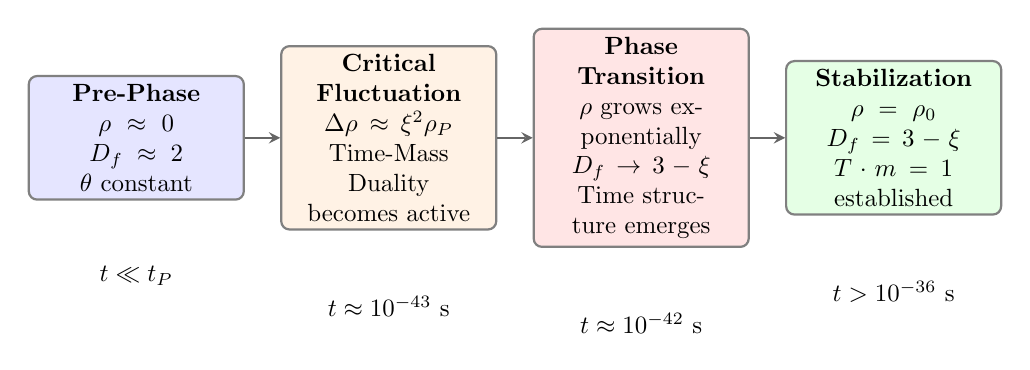
\begin{tikzpicture}[
			node distance=1cm and 0.5cm,
			phase/.style={rectangle, draw=black!50, thick, minimum width=3cm, minimum height=1.5cm, align=center, rounded corners=3pt, text width=2.8cm},
			arrow/.style={->, >=stealth, thick, black!60},
			scale=0.9,
			transform shape
			]
			
			% Phases in chronological order
			\node (pre) [phase, fill=blue!10] {\textbf{Pre-Phase} \\ $\rho \approx 0$ \\ $D_f \approx 2$ \\ $\theta$ constant};
			\node (fluk) [phase, fill=orange!10, right=of pre] {\textbf{Critical Fluctuation} \\ $\Delta\rho \approx \xi^2\rho_P$ \\ Time-Mass Duality \\ becomes active};
			\node (ubergang) [phase, fill=red!10, right=of fluk] {\textbf{Phase Transition} \\ $\rho$ grows exponentially \\ $D_f \to 3-\xi$ \\ Time structure emerges};
			\node (stabil) [phase, fill=green!10, right=of ubergang] {\textbf{Stabilization} \\ $\rho = \rho_0$ \\ $D_f = 3-\xi$ \\ $T \cdot m = 1$ established};
			
			% Time axis
			\node (zeit0) [below=0.3cm of pre, yshift=-0.5cm] {$t \ll t_P$};
			\node (zeit1) [below=0.3cm of fluk, yshift=-0.5cm] {$t \approx 10^{-43}$ s};
			\node (zeit2) [below=0.3cm of ubergang, yshift=-0.5cm] {$t \approx 10^{-42}$ s};
			\node (zeit3) [below=0.3cm of stabil, yshift=-0.5cm] {$t > 10^{-36}$ s};
			
			% Arrows
			\draw [arrow] (pre) -- (fluk);
			\draw [arrow] (fluk) -- (ubergang);
			\draw [arrow] (ubergang) -- (stabil);
			
		\end{tikzpicture}
	\end{center}
	
	\textbf{Detailed Chronology:}
	
	\begin{enumerate}
		\item \textbf{Pre-Vacuum (\(t < 10^{-43}\) s):}
		\begin{itemize}
			\item \(\rho \approx 0\), \(D_f \approx 2\)
			\item Pure phase field \(\theta\), constant and disordered
			\item Time-Mass Duality not yet active (since \(m \approx 0\))
			\item No measurable time, no measurable mass
		\end{itemize}
		
		\item \textbf{Critical Point (\(t \approx 10^{-43}\) s):}
		\begin{itemize}
			\item Fractal fluctuation reaches \(\Delta\rho \approx \xi^2\rho_P\)
			\item Time-Mass Duality becomes active: \(T \cdot m > 0\)
			\item Instability in potential \(V(\rho)\) becomes relevant
			\item Phase transition begins
		\end{itemize}
		
		\item \textbf{Exponential Growth (\(10^{-43} < t < 10^{-42}\) s):}
		\begin{itemize}
			\item \(\rho\) grows exponentially: \(\rho(t) \approx \Delta\rho \cdot e^{t/\tau}\)
			\item \(\tau = \hbar/(m_P c^2 \xi^2) \approx 10^{-43}\) s: Characteristic time
			\item \(D_f\) evolves from \(\approx 2\) to \(3-\xi\)
			\item Time emerges as phase evolution: \(d\tau \propto d\theta/\rho\)
		\end{itemize}
		
		\item \textbf{Stabilization (\(t > 10^{-36}\) s):}
		\begin{itemize}
			\item \(\rho\) reaches equilibrium: \(\rho_0 = \sqrt{\hbar c}/(l_P^{3/2} \xi^2)\)
			\item \(D_f\) stabilizes at \(3 - \xi \approx 2.999867\)
			\item Speed of light established: \(c = \sqrt{K_0/\rho_0} \cdot (1 - \xi/2)\)
			\item Time-Mass Duality established: \(T(x,t) \cdot m(x,t) = 1\)
		\end{itemize}
	\end{enumerate}
	
	\subsection{Emergence of Fundamental Quantities}
	
	\textbf{Time:}
	\begin{equation}
		d\tau = \frac{\hbar}{m_P c^2} \cdot \frac{d\theta}{\rho/\rho_0} \cdot \xi^{-1}
	\end{equation}
	Time emerges as the derivative of phase evolution, scaled with \(\xi^{-1}\).
	
	\textbf{Speed of Light:}
	\begin{equation}
		c = \sqrt{\frac{K_0}{\rho_0}} \cdot \left(1 - \frac{\xi}{2}\right) \approx 2.9979 \times 10^8 \, \text{m/s}
	\end{equation}
	The maximum signal speed emerges from vacuum stiffness \(K_0\).
	
	\textbf{Gravitation:}
	\begin{equation}
		G = \frac{c^3 l_P^2}{\hbar} \cdot \xi^2 \approx 6.674 \times 10^{-11} \, \text{m}^3\text{kg}^{-1}\text{s}^{-2}
	\end{equation}
	The gravitational constant emerges as a consequence of fractal spacetime structure.
	
	\textbf{Particle Masses:}
	\begin{equation}
		m_i = m_P \cdot f_i(\xi) \cdot \xi^{k_i}
	\end{equation}
	where \(f_i(\xi)\) are specific fractal form factors and \(k_i\) are hierarchy levels.
	
	\subsection{The Low Entropy Problem}
	
	The extremely low initial entropy of the observable universe (\(\sim 10^{88} k_B\)) is naturally explained in T0:
	
	\textbf{Initial Entropy:}
	\begin{equation}
		S_{\text{initial}} \approx k_B \cdot \ln\left(\frac{V_{\text{eff}}}{l_P^3}\right) \cdot \xi^3 \approx 10^{88} k_B
	\end{equation}
	
	\textbf{Explanation:}
	\begin{itemize}
		\item The pre-vacuum has nearly zero entropy through its fractal self-similarity
		\item Entropy only grows with the emergence of \(\rho > 0\)
		\item The factor \(\xi^3 \approx 2.37 \times 10^{-10}\) reduces the maximum possible entropy
		\item This explains the ``ordered'' initial state without fine-tuning
	\end{itemize}
	
	\subsection{Testable Consequences}
	
	\textbf{1. Fractal Signatures in CMB:}
	\begin{equation}
		\frac{\delta T}{T}(\vec{n}) \propto \xi \cdot \sum_{n} \frac{\cos(2\pi |\vec{x}_n|/\lambda_n)}{|\vec{x}_n|^{D_f/2}}
	\end{equation}
	The anisotropy patterns should show fractal self-similarity with scaling exponent \(D_f/2 \approx 1.5\).
	
	\textbf{2. Time Variation of \(\xi\):}
	\begin{equation}
		\left|\frac{\dot{\xi}}{\xi}\right| \approx 2.3 \times 10^{-18} \, \text{s}^{-1}
	\end{equation}
	This slow variation should be detectable in precision experiments with atomic clocks.
	
	\textbf{3. Modified Inflation:}
	Instead of a separate inflation phase:
	\begin{equation}
		a(t) \propto t^{2/D_f} \approx t^{0.6667} \quad \text{(early era)}
	\end{equation}
	This should be recognizable in the B-mode polarization spectrum of the CMB.
	
	\subsection{Comparison with Alternative Theories}
	
	\begin{center}
		\begin{tabular}{p{0.3\textwidth}|p{0.3\textwidth}|p{0.3\textwidth}}
			\textbf{Aspect} & \textbf{Loop Quantum Cosmology (LQC)} & \textbf{Fractal T0-Cosmology} \\
			\hline
			Pre-Phase & Quantum geometry with Immirzi parameter \(\gamma\) & Fractal zero-vacuum with \(D_f \approx 2\) \\
			Transition & Big Bounce at \(\rho = \rho_{\text{crit}}\) & Phase transition at \(\rho \approx \xi^2\rho_P\) \\
			Parameters & \(\gamma \approx 0.2375\), \(\rho_{\text{crit}}\) & Only \(\xi = \frac{4}{3} \times 10^{-4}\) \\
			Dimensions & 3+1 & 3+1 with fractal structure \(D_f = 3-\xi\) \\
			Entropy Problem & Requires special initial conditions & Naturally explained by \(\xi^3\) factor \\
			\hline
			\textbf{Aspect} & \textbf{String Theory Cosmology} & \textbf{Fractal T0-Cosmology} \\
			\hline
			Pre-Phase & Higher-dimensional branes/compactification & Fractal 4D zero-vacuum \\
			Transition & Brane collision/tunneling & Deterministic phase transition \\
			Parameters & Many (moduli, dilaton, etc.) & Only \(\xi\) \\
			Dimensions & 10-11 (must be compactified) & 3+1 with fractal structure \\
			Predictions & Complex, multiverse & Precise, testable deviations \\
		\end{tabular}
	\end{center}
	
	\subsection{Philosophical Implications}
	
	The T0-chronology has profound philosophical consequences:
	
	\begin{itemize}
		\item \textbf{No Singularity}: The ``beginning'' is a regular physical transition, not a mathematical singularity
		\item \textbf{Deterministic}: The transition inevitably follows from the Time-Mass Duality and \(\xi\)
		\item \textbf{Parameter-free}: Only \(\xi\) as fundamental parameter, all other quantities emerge
		\item \textbf{Static Universe}: No expansion, only fractal deepening
		\item \textbf{Natural Fine-Tuning}: The ``fine-tuned'' constants arise naturally from \(\xi\)
	\end{itemize}
	
	\subsection{Conclusion}
	
	The chronology of universe creation in T0-theory offers the simplest and most parameter-sparse description of cosmological origin:
	
	\begin{itemize}
		\item \textbf{One Parameter}: Everything emerges from \(\xi = \frac{4}{3} \times 10^{-4}\)
		\item \textbf{No Singularity}: Big Bang as regular fractal phase transition with minimal core scale $L_0$ (from $\xi$)
		\item \textbf{Time-Mass Duality as Driver}: \(T(x,t) \cdot m(x,t) = 1\) drives the transition
		\item \textbf{Natural Explanation for Fine-Tuning}: All ``fine-tuned'' constants follow from \(\xi\)
		\item \textbf{Testable Predictions}: Fractal patterns in CMB, time variation of fundamental constants
	\end{itemize}
	
	Instead of an explosive beginning from a singularity, T0 describes a smooth, deterministic transition from a minimal fractal state. The universe doesn't ``begin'' in the conventional sense, but unfolds from a highly symmetric pre-phase through the self-consistent dynamics of the Time-Mass Duality.
	
	This view not only eliminates the problem of the initial singularity, but also provides a natural explanation for the puzzling fine-tuning of natural constants and the extremely low initial entropy of the cosmos – all emergent consequences of the single fundamental parameter \(\xi\).
	
\end{document}
